\newcommand{\uL}{\mathbf{L_0}}
\newcommand{\bL}{\mathbf{\bar{L}_0}}
\begin{block}{CFT Identification}
\begin{columns}[T]
\begin{column}{.3\textwidth}

%\begin{table}[h]
\begin{tabular}{lr}

$\mathbf{P} =\frac{2\pi}{L}(\uL-\bL)$ & 
$\frac{2\pi}{L}(em + n - \bar{n})$ \\
&
\\
$\widetilde{\mathbf{P}}$  &
$(em + n - \bar{n})$\\
& 
\\
$\mathbf{H} = \frac{2\pi}{L}(\uL+\bL)$ &
 $\frac{2\pi}{L}(\frac{\kappa e^2}{2} + \frac{m^2}{2 \kappa} + \frac{n + \bar{n}}{2})$ \\
&
 \\
$\widetilde{\mathbf{H}} = \frac{L}{2 \pi \kappa}\mathbf{H}$ &
 $e^2 + \frac{m^2}{4 \kappa^2} + \frac{1}{\kappa}(n + \bar{n})$       
\end{tabular}
%\label{Table:EV}
%\caption{Eigenvalues of states $\ket{e, m}_{n, \bar{n}}$.} 
%\end{table}

\end{column}
\begin{column}{.5\textwidth}
\vskip-1cm
\begin{figure}[hbctp]
\begin{center}
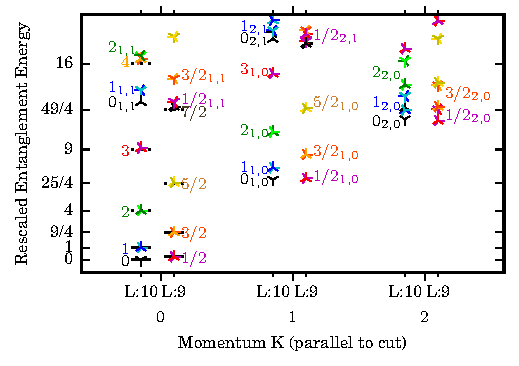
\includegraphics{{interpolatedboson/a10/plots/EEIdentify.pdf}}
\end{center}
%\caption{The identification of the states $\ket{e, m}_{n, \bar{n}}$ in the spectrum of the soft-core boson entanglement Hamiltonian. The label $e$ gives the U(1) charge. The labels $n$, $\bar{n}$ label the levels in the right or left-moving sectors of the Kac-Moody algebra. When the level $n$ is larger than 1, the level shows $Z(n)$ approximately degenerate states. The best estimate for the Luttinger parameter $\kappa = 1/6.4$ is given by the inverse of the energy of the $\ket{1, 0}_{1, 0}$ state. The label $m$ is 0 for all states shown - however, the primary states $\ket{e, m=\pm 1}$ can be seen centered around momentum $\pi$, with energies on the order of $1/(4\kappa^2)$.}
%\label{fig:primaries}
\end{figure}

\end{column}
\end{columns}
\end{block}